\section{Struktura danych \textsc{CDLMW SF}}
\label{sec:sf}
Przedstawimy strukturę danych (algorytm 3 z pracy \cite{chan14}), którego czas działania jest wrażliwy na liczbę unikalnych elementów $\dt$. Wspiera ona jedną operacje -- $\textsc{query}(i,j)$ -- zwracającą dominantę $A[i:j]$, w czasie $\Oh(\dt)$.
\subsection{Konstrukcja}
\begin{figure}[H]
    \centering
    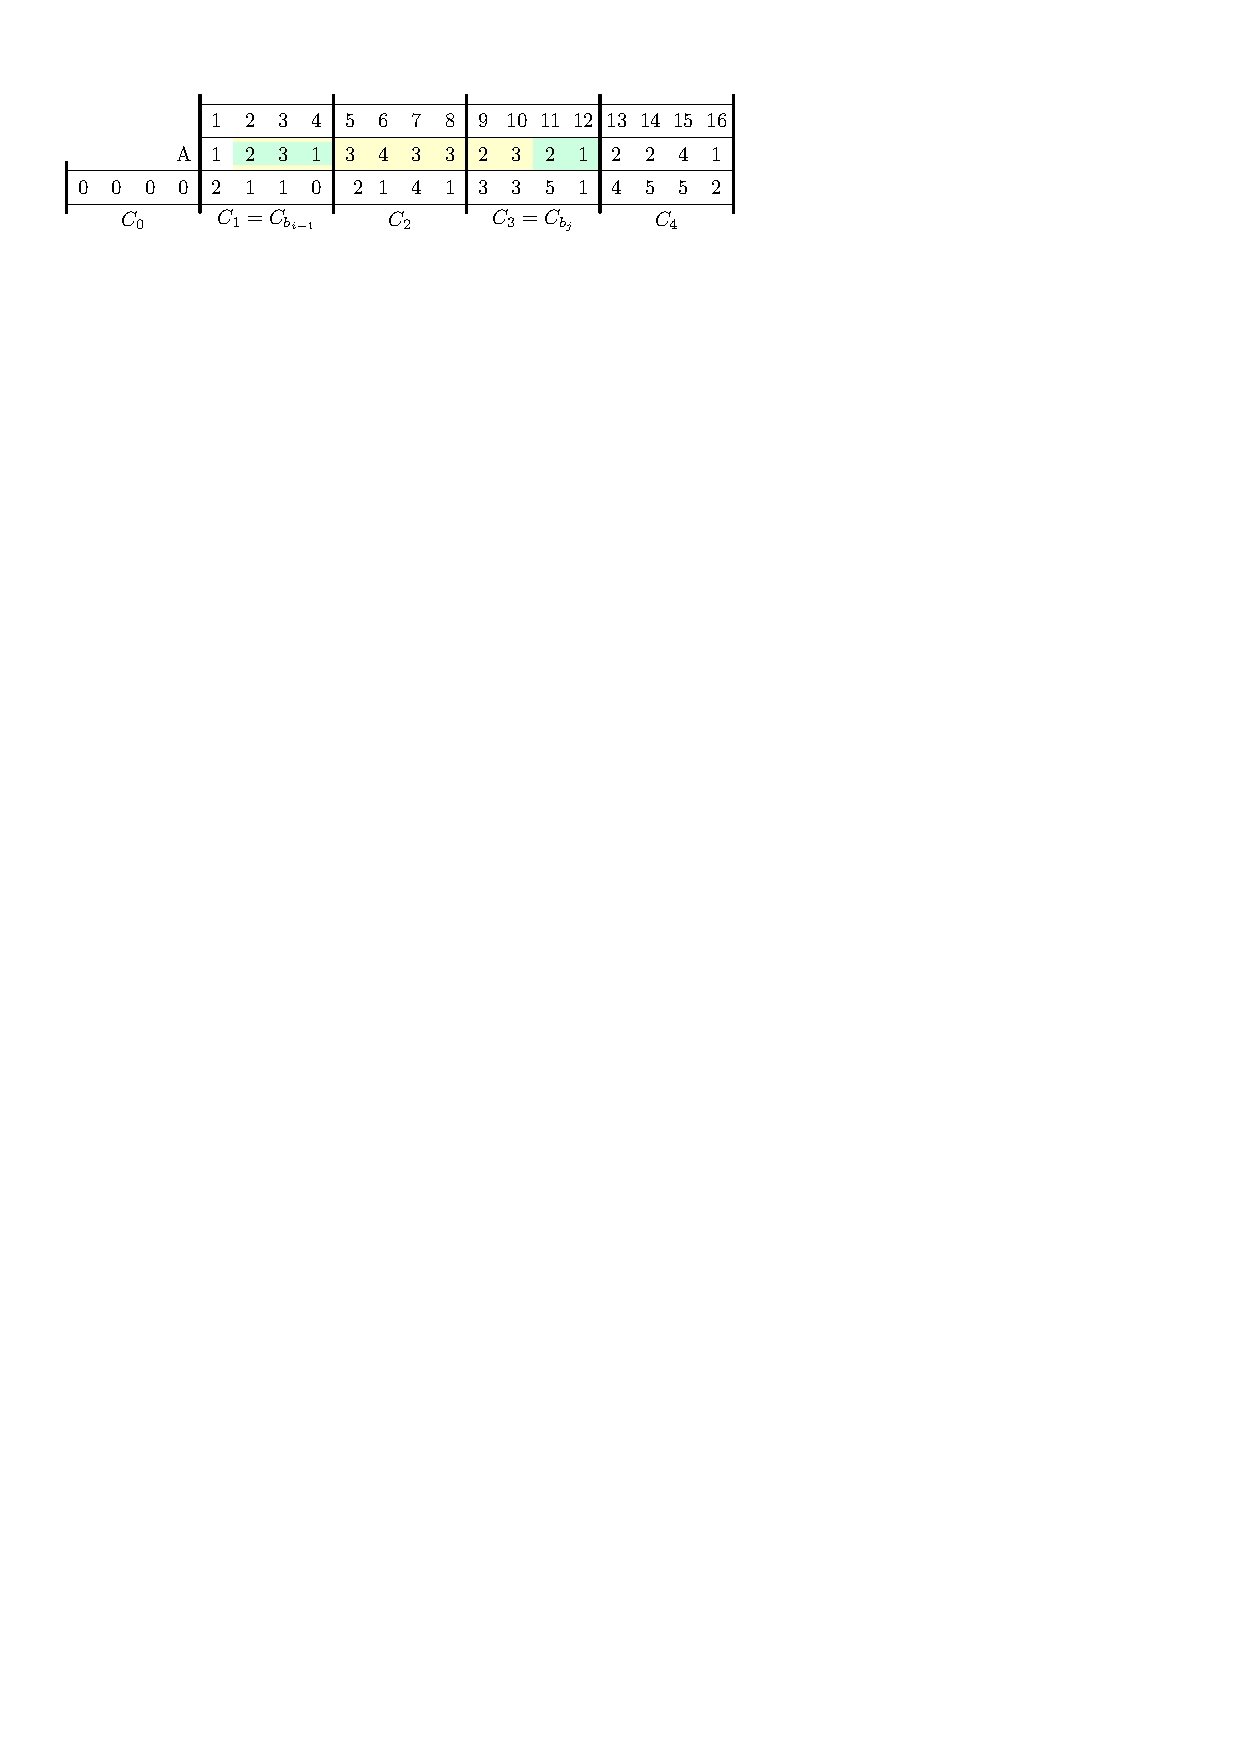
\includegraphics[scale=1.1]{images/sf.pdf}
    \caption{
    Przykładowa tablica $A[1:16]$ z liczbą unikalnych elementów $\dt=4$ i podziałem na $s=4$ bloki, każdy o rozmiarze $t=4$. Ponadto zaznaczamy zapytanie o dominantę $A[2:10]$, prefiks $A[2:4]$ oraz sufiks $A[11:12]$, które są zaznaczone kolorem żółtym, zielonym oraz zielonym. Dodatkowo $C_1=C_{b_{i-1}}$ oraz $C_3 = C_{b_j}$}
    \label{fig:sparse_freq_tbl}
\end{figure}
  Dzielimy tablicę $A$ na bloki o rozmiarze $\dt$, przy czym dopuszczamy by ostatni blok miał mniejszy rozmiar. Dla każdego $i \in \{0, ..., \cl{\frac n \dt}\}$ tworzymy tablicę $C_i[1:\dt]$, która na $j$-tej pozycji zawiera liczbę wystąpień wartości $j$ w pierwszych $i$ blokach. Innymi słowy, $C_i[j]$ to liczba wystąpień wartości $j$ w przedziale $A[1:\min\{n, i\dt\}]$. Rysunek \ref{fig:sparse_freq_tbl} przedstawia przykładową tablicę i podział na bloki o rozmiarze $\dt=4$.
\subsection{Operacja \textsc{query}}
\begin{algorithm}[H]
    \caption{Operacja \textsc{query}}
    % \label{alg:sparse-freq-tbl-qry}
    \begin{algorithmic}[1]
        \Function{SFQuery}{$i$, $j$}
            \State Niech $C[1:\dt]$ będzie tymczasową tablicą.
            \State $b_{i-1} \gets \cl{(i-1)/\dt}$
            \State $b_j \gets \cl{j/\dt}$
            \For{$k \gets 1,\dots,\dt$}
                \State $C[k] \gets C_{b_j}[k] - C_{b_{i-1}}[k]$
            \EndFor
            \State prefiks $\gets \min(n,b_{i-1}\dt)$
            \For{$k \gets i,\dots,$prefiks}
                \State $C[A[k]] \gets C[A[k]]+1$
            \EndFor
            \State sufiks $\gets \min(n, b_j\dt)$
            \For{$k \gets j+1,\dots,$sufiks}
                \State $C[A[k]] \gets C[A[k]]-1$
            \EndFor
            \State mode $\gets \argmax C$
            \State \Return C[mode], mode
        \EndFunction
    \end{algorithmic}
\end{algorithm}
Rozważmy zapytanie o dominantę na przedziale $A[i:j]$. Niech $b_j=\cl{j / \dt}$ oraz $b_{i-1}=\cl{(i-1) / \dt}$ to indeksy bloków, do których należą odpowiednio wartości $A[j]$ oraz $A[i-1]$. Zauważmy że częstotliwość wszystkich elementów na przedziale $A[b_{i-1}\dt+1:b_j\dt]$ możemy obliczyć przez odjęcie $C_{b_{i-1}}$ od $C_{b_j}$. Oznaczmy różnicę tych dwóch tablic przez $C$. Aby uzyskać częstotliwość wszystkich elementów na przedziale $A[i:j]$ trzeba uwzględnić brakujące wartości $A[b_{i-1}\dt:i]$ oraz nadmiarowe wartości $A[j+1:b_j\dt]$ ($A[j+1:n]$, gdy $b_j$ jest ostatnim blokiem). Nazwijmy brakujące elementy prefiksem, a nadmiarowe elementy sufiksem. Elementów prefiksu i sufiksu nie jest zbyt wiele, dlatego przeglądamy je po kolei aktualizując ich częstotliwość w tablicy $C$.
\subsection{Analiza złożoności pamięciowej}
Przechowujemy $1+\cl{n/\dt}$ tablic $C_i$, każda o rozmiarze $\dt$. W trakcie obliczania dominanty posługujemy się roboczą tablicą o rozmiarze $\dt$. Łącznie zużywamy $\left(1+\cl{n/\dt}\right)\dt + \dt \in \Oh(n)$ pamięci.
\subsection{Analiza złożoności czasowej}
Obliczenie różnicy $C_{b_j} - C_{b_{i-1}}$ zajmuje czas $\Oh(\dt)$. Rozmiar prefiksu i sufiksu możemy ograniczyć od góry przez $\dt-1$, zatem dodanie elementów prefiksu i odjęcie elementów sufiksu łącznie zajmie $\Oh(\dt)$ czasu. W takim razie operacje zapytania, łącznie zajmują czas $\Oh(\dt)$.
\subsection{Implementacja}
\label{sec:cdlmw-sf-impl}
Dzięki temu że tablice $C_{b_{i-1}}$ oraz $C_{b_j}$ zajmują ciągły fragment pamięci, możemy łatwo zwektoryzować obliczanie ich różnicy. W naszej implementacji używamy instrukcji wektorowej \lstinline{_mm512_sub_epi64}\footnote{\url{ https://software.intel.com/sites/landingpage/IntrinsicsGuide/\#text=_mm512_sub_epi64}}, która pozwala na odjęcie 4 wartości $64$bitowych na raz. Instrukcja ta jest dostępna na większości nowych procesorów Intel oraz AMD.\\
\\
W zależności od rozmiaru sufiksu możemy uzyskać lepszy praktyczny czas działania, obsługując sufiks inaczej. Zauważmy, że zamiast uwzględniać cały blok $b_j$ i potem odejmować od niego sufiks, równoważnie możemy go zignorować i dodać elementy $A[(b_j-1)\dt+1:j]$. W przypadku gdy sufiks $A[j+1:b_j\dt]$ jest mniejszy niż $\cl{\dt/2}$ używamy oryginalnego przetwarzania, a w przeciwnym przypadku używamy nowego. Dzięki temu pesymistycznie będziemy musieli przeskanować $\cl{\dt/2}$ zamiast $\dt-1$ elementów. Analogiczną optymalizacje możemy zastosować do skanowania prefiksu. Łącznie pesymistycznie będziemy musieli przeskanować $2\cl{\dt/2}$ elementów zamiast $2\dt-2$.
\newpage